\chapter{Wyniki}
\label{ch:wyniki}

% TODO: prezentacja i omówienie wyników przeprowadzonych badań.

\section{Płytka z~diodą LED}
\label{sec:wyniki-led}

Pierwsza płytka testowa jest prostym układem zaprojektowanym samodzielnie
w~EasyEDA. Zawiera cztery elementy: gniazdo baterii (B1), przycisk (SW1),
rezystor (R1) i~diodę LED (LED1), które mają łącznie 10~padów
powierzchniowych (SMD). Płytka ma wymiary $51 \times 34$~mm
($2008 \times 1339$~mil), dwie warstwy sygnałowe i~cztery sieci dwupinowe,
co daje cztery połączenia do poprowadzenia.

Wyniki trasowania płytki w~trzech badanych wariantach przedstawiono na
rysunkach~\ref{rys:led-easyeda}--\ref{rys:led-unet}, a~ich
parametry zestawiono w~tabeli~\ref{tab:wyniki-led}. Ścieżki na warstwie
górnej oznaczono kolorem czerwonym, a~na warstwie dolnej --- niebieskim.

\begin{figure}[H]
\centering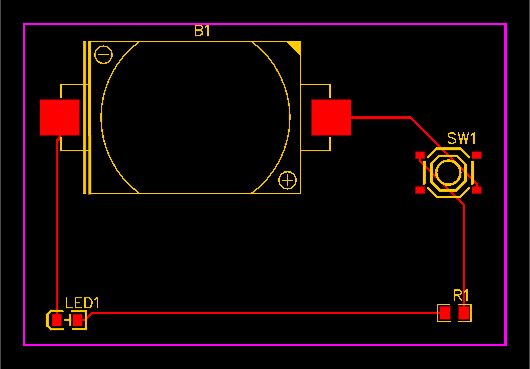
\includegraphics[width=0.8\textwidth]{figures/PCB_PCB_Magisterka_2_2026-11-15}
\caption{Płytka z~diodą LED poprowadzona autorouterem EasyEDA. Źródło:
opracowanie własne.}\label{rys:led-easyeda}
\end{figure}

Autorouter EasyEDA poprowadził wszystkie cztery sieci wyłącznie na warstwie
górnej, bez użycia przelotek. Łączna długość ścieżek wynosi 98,44~mm.
Ścieżki składają się z~odcinków poziomych, pionowych i~nachylonych pod kątem
45°, a~każde połączenie ma tylko kilka załamań. Sprawdzenie reguł
projektowych (DRC) nie wykazało naruszeń.

\begin{figure}[H]
\centering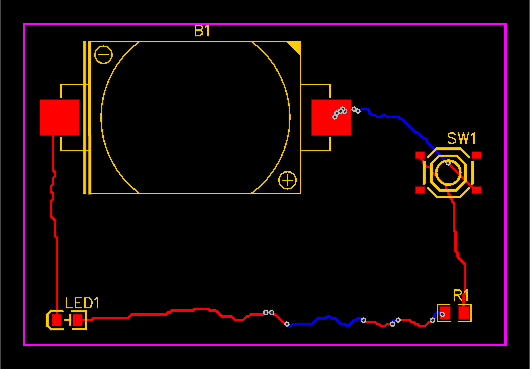
\includegraphics[width=0.8\textwidth]{figures/PCB_PCB_Magisterka_3_2026-11-15}
\caption{Płytka z~diodą LED poprowadzona algorytmem A* bez sieci neuronowej.
Źródło: opracowanie własne.}\label{rys:led-astar}
\end{figure}

Algorytm A* również poprowadził wszystkie cztery sieci, a~DRC nie wykazało
naruszeń reguł projektowych. Łączna długość ścieżek wynosi 106,79~mm, czyli
o~8,5\% więcej niż w~wariancie EasyEDA. Ścieżki wielokrotnie przechodzą
między warstwami, co dało 16~przelotek wobec braku przelotek w~wariancie
EasyEDA. Przebieg ścieżek jest nieregularny: na trasie występuje wiele
drobnych załamań, wynikających z~prowadzenia ścieżek po siatce o~boku
8~mil z~ruchami po przekątnej. Trasowanie trwało 15,0~s, a~algorytm
rozwinął 121\,772~węzły.

\begin{figure}[H]
\centering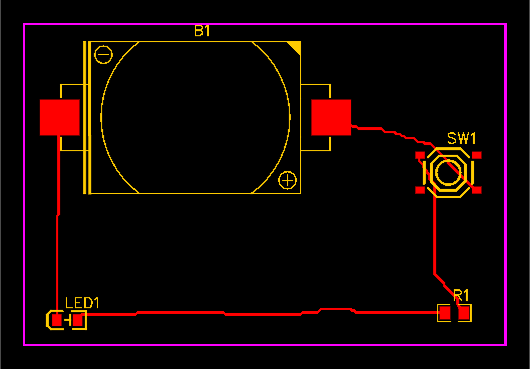
\includegraphics[width=0.8\textwidth]{figures/PCB_PCB_Magisterka_UnetAstar_2026-11-16}
\caption{Płytka z~diodą LED poprowadzona algorytmem Unet-A*. Źródło:
opracowanie własne.}\label{rys:led-unet}
\end{figure}

Algorytm Unet-A* poprowadził wszystkie cztery sieci wyłącznie na warstwie
górnej, bez użycia przelotek, a~DRC nie wykazało naruszeń reguł
projektowych. Łączna długość ścieżek wynosi 100,02~mm. Jest to o~1,6\% więcej
niż w~wariancie EasyEDA i~o~6,3\% mniej niż w~wariancie A*. Przebieg
połączeń jest niemal taki sam jak w~wariancie EasyEDA
(rys.~\ref{rys:led-easyeda}): ścieżki biegną tą samą drogą od gniazda baterii
przez diodę, rezystor i~przycisk. Różnią się jednak kształtem. Zamiast
prostych odcinków mają drobne, schodkowe załamania wynikające z~prowadzenia
po siatce, choć jest ich mniej niż w~wariancie A*.
Trasowanie trwało 4,6~s, czyli ponad trzykrotnie krócej niż w~wariancie A*.
Algorytm rozwinął 61\,582~węzły, o~49\% mniej niż A*.

\begin{table}[ht]
\fcmtcaption{Parametry płytki z~diodą LED w~badanych wariantach. Źródło:
opracowanie własne.}\label{tab:wyniki-led}
\centering\footnotesize%
\begin{tabular}{l r r r}
\toprule
Miara & EasyEDA & A* & Unet-A* \\
\midrule
Połączone sieci & 4/4 & 4/4 & 4/4 \\
\midrule
Długość ścieżek [mm] & 98,44 & 106,79 & 100,02 \\
\midrule
Liczba przelotek & 0 & 16 & 0 \\
\midrule
Naruszenia DRC & 0 & 0 & 0 \\
\midrule
Czas trasowania [s] & --- & 15,0 & 4,6 \\
\midrule
Rozwinięte węzły & --- & 121\,772 & 61\,582 \\
\bottomrule
\end{tabular}
\end{table}

\section{Płytka przykładowa EasyEDA}
\label{sec:wyniki-sample}

Druga płytka testowa pochodzi z~przykładowego projektu (\emph{Sample Project})
udostępnionego w~sekcji \emph{Modules} serwisu
EasyEDA~\cite{EasyEDA_ProjectSample}. Zawiera osiem elementów:
złącze (U1), dwa tranzystory (Q1, Q2), kondensator (C1) i~cztery rezystory
(R1--R4). Elementy mają łącznie 29~padów, z~czego 18~to pady powierzchniowe
(SMD), a~11~pady przewlekane (THT). Płytka ma wymiary $37 \times 25$~mm
i~dwie warstwy sygnałowe. Projekt zawiera sześć sieci.

Wyniki trasowania przedstawiono na
rysunkach~\ref{rys:sample-easyeda}--\ref{rys:sample-unet}, a~ich parametry
zestawiono w~tabeli~\ref{tab:wyniki-sample}.

\begin{figure}[H]
\centering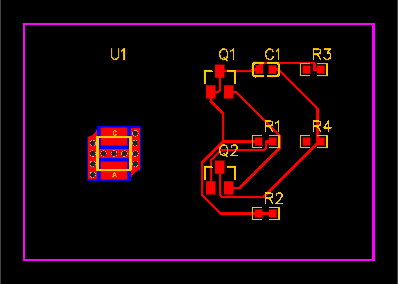
\includegraphics[width=0.8\textwidth]{figures/PCB_PCB_SamplePCB_2026-11-15}
\caption{Płytka przykładowa EasyEDA poprowadzona autorouterem EasyEDA.
Źródło: opracowanie własne.}\label{rys:sample-easyeda}
\end{figure}

Autorouter EasyEDA poprowadził cztery z~sześciu sieci. Niepoprowadzone
pozostały połączenia złącza U1 z~resztą układu. Wszystkie ścieżki leżą na
warstwie górnej, bez przelotek, a~ich łączna długość wynosi 92,51~mm.
DRC wykazało dwa naruszenia reguł projektowych. Oba dotyczą
niedokończonych połączeń, czyli dwóch sieci, których autorouter nie
poprowadził.

\begin{figure}[H]
\centering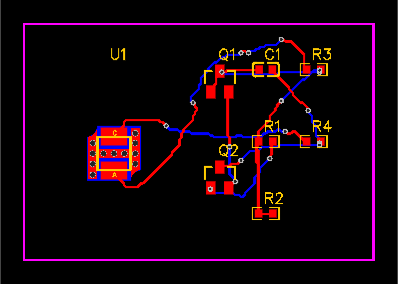
\includegraphics[width=0.8\textwidth]{figures/PCB_PCB_SamplePCB_2026-11-15_2}
\caption{Płytka przykładowa EasyEDA poprowadzona algorytmem A* bez sieci
neuronowej. Źródło: opracowanie własne.}\label{rys:sample-astar}
\end{figure}

Algorytm A* poprowadził wszystkie sześć sieci, łącznie z~połączeniami
złącza U1, a~DRC nie wykazało naruszeń reguł projektowych. Ścieżki
prowadzone są na obu warstwach, co wymagało 18~przelotek. Łączna długość
ścieżek wynosi 149,29~mm, czyli o~61\% więcej niż w~wariancie EasyEDA.
Długości nie są jednak w~pełni porównywalne, ponieważ wariant EasyEDA nie
zawiera dwóch niepoprowadzonych sieci. Podobnie jak na płytce z~diodą LED,
ścieżki mają nieregularny przebieg z~wieloma drobnymi załamaniami.

\begin{figure}[H]
\centering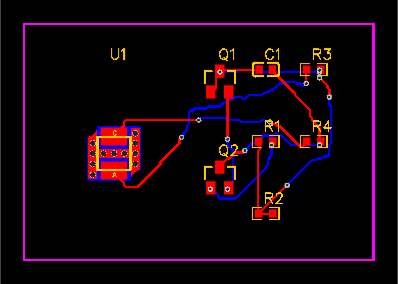
\includegraphics[width=0.8\textwidth]{figures/PCB_PCB_SamplePCB_UnetAstar_2026-11-16}
\caption{Płytka przykładowa EasyEDA poprowadzona algorytmem Unet-A*.
Źródło: opracowanie własne.}\label{rys:sample-unet}
\end{figure}

Algorytm Unet-A* również poprowadził wszystkie sześć sieci, łącznie
z~połączeniami złącza U1. DRC nie wykazało naruszeń reguł projektowych.
Ścieżki prowadzone są na obu warstwach, co wymagało 16~przelotek, o~dwie
mniej niż w~wariancie A*. Łączna długość ścieżek wynosi 146,44~mm. Jest to
o~1,9\% mniej niż w~wariancie A*, ale o~58\% więcej niż w~wariancie EasyEDA.
Tę ostatnią różnicę należy jednak interpretować ostrożnie, ponieważ wariant
EasyEDA nie zawiera dwóch sieci. Kształt ścieżek jest podobny jak
w~wariancie A*: występują drobne załamania wynikające z~prowadzenia po
siatce. Trasowanie trwało 3,1~s wobec 16,6~s dla A*, a~liczba rozwiniętych
węzłów spadła ze 160\,493 do 45\,516, czyli o~72\%.

\begin{table}[ht]
\fcmtcaption{Parametry płytki przykładowej EasyEDA w~badanych wariantach.
Źródło: opracowanie własne.}\label{tab:wyniki-sample}
\centering\footnotesize%
\begin{tabular}{l r r r}
\toprule
Miara & EasyEDA & A* & Unet-A* \\
\midrule
Połączone sieci & 4/6 & 6/6 & 6/6 \\
\midrule
Długość ścieżek [mm] & 92,51 & 149,29 & 146,44 \\
\midrule
Liczba przelotek & 0 & 18 & 16 \\
\midrule
Naruszenia DRC & 2 & 0 & 0 \\
\midrule
Czas trasowania [s] & --- & 16,6 & 3,1 \\
\midrule
Rozwinięte węzły & --- & 160\,493 & 45\,516 \\
\bottomrule
\end{tabular}
\end{table}
